\chapter{Defensive Points-To Analysis}
\label{chapter:defensive}
\epigraph{You don’t just give up. You don’t just let things happen. You make a stand!}{\textit{Rose Tyler} - Doctor Who}
%\epigraph{Progress isn't made by early risers. It's made by lazy men trying to find easier ways to do something.}{\textit{Robert Heinlein}}

\emph{Soundness} is a coveted property of static analyses, to the extent that the term is often colloquially used as a synonym for ``correctness''. For a may-analysis, soundness means that the analysis abstraction overapproximates all concrete executions. A sound value-flow or points-to analysis is one that computes, per program point or per variable, value sets that represent (at least) all values that could possibly arise at the respective point during any possible execution.

Full soundness is hard to achieve in practice due to code that cannot be analyzed (e.g., dynamically generated/loaded code, binary/native code) or dynamic language features (e.g., reflection, \code{eval}, \code{invokedynamic}). We collectively refer to such features as \emph{opaque code}. For instance, the Java code below invokes an unknown method, identified by string \code{methodName}, over an object, \code{obj}.

\begin{javaBox}
Method m = obj.getClass().getMethod(methodName);
m.invoke(obj);  
\end{javaBox}

String \code{methodName} could be a true run-time value---e.g., read from a file or external resource. Object \code{obj} could itself be of a type not available during analysis---e.g., \code{obj} could be obtained through the network and statically typed using a vague interface or root-of-hierarchy type.

Faced with such complications, all past analyses that claim soundness have done so under \emph{a priori} qualifications. Prominently, abstract-interpretation-based~\cite{popl:1977:Cousot} approaches, such as Astr\'{e}e~\cite{sas:2007:Delmas}, have long emphasized soundness. The conceptual form of such a soundness result is as follows:\footnote{This formulation is due to Xavier Rival of the Astr\'{e}e project (e.g., \cite{misc:Xavier}).}

\begin{quote}
An $Analysis$ of programs in language $Lang$ is sound relative to language subset $Lang'$ and executions set $Exec'$ iff:

\hspace{8 mm} $\forall$ program $P \in Lang$: $P \in Lang' \land e \in Exec' \implies e \in \gamma(Analysis(P))$

(where $\gamma$ is the concretization function that maps abstractions in the output domain of $Analysis$ to concrete executions in a universe $Exec$, superset of $Exec'$).
\end{quote}

The problem with this formulation of soundness is that, although it yields provable theorems, the \emph{a priori} qualification excludes virtually all realistic programs. The $Lang'$ or $Exec'$ of published proofs disqualify the vast majority of modern programs ``in the wild''. Language subset $Lang'$ will typically exclude all dynamic features (e.g., reflection) and/or executions subset $Exec'$ will disqualify all behaviors that are deemed too-dynamic (e.g., invoking dynamically-loaded code). Reflection alone disqualifies $\sim$80\% of Java programs in the 461-program corpus of the recent Landman et al. study~\cite{icse:2017:Landman}.

The above issues have led several members of the static analysis community to proclaim that ``\emph{all published whole-program analyses are unsound}''~\cite{article:2015:Livshits}, i.e., their soundness guarantee does not apply to realistic programs, and similarly that ``\emph{[there is not] a single realistic whole-program analysis tool [...] that does not purposely make unsound choices}''. The problem is, therefore, both theoretical and practical. Soundness theorems do not give guarantees for realistic programs. Implementations of analyses in tools happily perpetuate the illusion: they handle soundly the language features one can prove theorems about, while cutting corners in the sound handling of all \emph{other} features, in order to demonstrate greater scalability or precision. For instance, in our earlier Java code fragment, even if the type of \code{obj} is known, many implemented static analyses will not consider all its methods (which now form a small finite set) as possible values of \code{m}, but will instead ignore the code altogether. This phenomenon has led to the introduction of the term \emph{soundy}~\cite{article:2015:Livshits} to characterize such analyses (recall Section~\ref{sec:back:soundiness}). Despite the derogatory tone, ``soundy'' analyses are the current \emph{good} case of static analyses! They are realistic analyses that handle all ``normal'' language features soundly.

In this work, we propose \emph{defensive analysis}: a static analysis architecture that addresses the above soundness shortcomings. The basis of defensive analysis can be seen as a different conceptual formulation of soundness.

\begin{quote}
An $Analysis$ of program $P$ in language $Lang$ computes results, $Analysis(P)$, together with soundness marker sets, $Claim(P)$. The $Analysis$ is sound iff:

\hspace{8 mm} $\forall$ program $P \in Lang$, execution $e$: $e[Claim(P)] \in \gamma(Analysis(P))[Claim(P)]$

(where $\gamma$ is as before, and $e[Claim(p)]$ is the restriction of an execution $e$ to program points with soundness claims, and the definition is similarly lifted to sets of executions).
\end{quote}

In other words, the analysis imposes no (or very liberal) \emph{a priori} restrictions to its soundness claims, but instead \emph{computes} the claimed domain of its soundness: the program parts for which the analysis result is sound. The soundness theorem applies to all (or most) programs, under all execution conditions---instead of eagerly disqualifying the vast majority of real-world programs. The extent of soundness is now defined over program points and becomes an experimentally measurable quantity: the size of $Claim(P)$ (which we term the \emph{coverage} of the analysis) can be measured to quantify for which percentage of a program's points the analysis is guaranteed to produce sound results.

The challenge of defensive analysis is, thus, to distinguish parts of the program that are certain to not be affected by opaque code. Delineating ``safe'' from ``unsafe'' parts of the program is an ambitious goal, since opaque code can do virtually anything: it can add dynamically-generated subclasses with never-seen methods that get called (via dynamic dispatch or first-class functions) at unsuspecting program points; it can call any existing method or alter any field via reflection; it can interpose its own implementations at every place where the program uses a reflective lookup; worst of all, it can wreak havoc on all parts of the heap reachable from any reference that escapes into opaque code.

To achieve the goal of distinguishing ``safe'' inferences, defensive analysis has a different logical form from past analyses. Instead of adding sophisticated handling of opaque code, defensive analysis redefines the analysis logic for regular, common language features, to defensively protect against the possibility that the analysis information potentially depends on opaque code. In essence, a defensive analysis produces inferences only when these are guaranteed to hold because of existing code and language features, and cannot possibly be violated by other, unknown code. Although this seems like a straightforward mode of operation, applying it to yield a realistic static analysis with useful coverage is a challenge.

We designed and implemented a defensive may-point-to (henceforth just ``points-to'') analysis for Java. The analysis follows the above form, explicitly designating points-to sets that are sound, i.e., that contain at least all the values that may ever arise in actual executions. Soundness guarantees carry over to the implementation: the soundness proof explicitly models all other language features as \unknown{} instructions and makes only weak, semantically-justified assumptions (e.g., a type-safe heap) about them. Soundness reasoning is defensive in that it establishes when the analysis can be certain to know the full contents of a points-to set, no matter what opaque code can do (within the stated weak assumptions).

In our effort to implement defensive analysis in a realistic package, we found \emph{laziness} to be an essential feature---the analysis cannot scale without it for real-world programs. Laziness means that the analysis does not compute points-to sets unless it can also claim their soundness. That is, program points outside of the $Claim(P)$ set do not get populated at any point---they remain empty throughout the analysis. Consequently, all points-to sets with a potentially unbounded number of objects (e.g., sets that depend on reflection or dynamic loading) are represented as the \emph{empty set}: the analysis never computes any contents for them. An empty analysis result merely means ``I don't know'', which could signify that the points-to set is affected by opaque code, or simply that the analysis cannot establish that it is \emph{not} affected by opaque code. Laziness yields high efficiency: the analysis can fall-back to an empty set (i.e., implicitly unbounded) without performing any computation or occupying space. 

The defensive nature of the analysis combined with laziness result in a very simple specification. The analysis does not need to integrate complex escape or alias reasoning (i.e., ``can this object \emph{ever} escape into opaque code?''), but only best-effort logic (i.e., ``here are simple, safe cases, when the object cannot possibly be affected by opaque code''). Failure to establish non-escaping merely means that the points-to set remains empty, to denote ``I don't know'' or ``potentially unbounded''.

In terms of applications, soundness is a requirement for ambitious clients, such as automatic optimization or semantics-preserving refactoring. Such clients are simply not feasible with past approaches. In particular, inter-procedural automatic optimization has long been hindered by the absence of sound points-to analysis information. Thus, our work has significant potential for wide practical application.

Concretely, in this chapter we describe the following:

\begin{itemize}
\item We offer a general static may-point-to analysis that yields sound results for realistic programs in the presence of opaque code. (Arguably other approaches \cite{ecoop:2004:Hirzel,article:2007:Hirzel,pldi:2007:Lattner} achieve soundness, but not for the full problem. Additionally, an analysis can be nominally sound by rejecting wholesale any program that employs features that the analysis does not handle. This is also not a solution. We compare more thoroughly in Section~\ref{sec:related:defensive} of related work.)

\item The analysis is efficient, leveraging its lazy representation of points-to sets. As a result, it can be made precise, beyond the limits of standard whole-program points-to analyses---e.g., for a 5-call-site-sensitive and flow-sensitive analysis. The analysis is also modular: it can be applied to any subset of the program, and will merely leave more points-to sets empty if other parts are unknown.
  
\item We show that the analysis, though quite defensive, yields useful coverage. In measurements over large Java benchmarks, our analysis computes guaranteed overapproximate points-to sets ($Claim(P)$) for 34-74\% of the local variables of a conventional unsound analysis. (This number is much higher than that of a conventional sound but intra-procedural analysis.) Similar effectiveness is achieved for other metrics (e.g., number of calls de-virtualized), again with actionable, guaranteed-sound outcomes.

\item The work brings some clarity to the domain of static analysis of opaque code. The approach allows, for the first time, to quantitatively weigh the benefits of sound inter-procedural analysis against its costs.
\end{itemize}


\section{Analysis Illustration}

We next describe the setting of defensive analysis and illustrate its principles and behavior.

\subsection{Soundness and Design Decisions}

Defensive analysis is a may-point-to analysis based on access paths, i.e., expressions of the form ``\texttt{\args{var}(\args{.fld})}*''). That is, the analysis computes \emph{the abstract objects} (i.e., allocation sites in the program text) \emph{that an access path may point to}. The analysis is flow-sensitive, hence we will be computing separate points-to information per program point. Both of these design decisions are integral elements of the analysis, as we will justify in Section~\ref{sec:sound:principles}.

Soundness in this setting means that the analysis computes an over-approximation of any points-to set---i.e., the analysis computes (abstractions of) all objects that may occur in an actual execution. However, since not all allocation sites are statically known (due to dynamically loaded code), such an over-approximation cannot be explicit: not all possible values in a points-to set can be listed. Thus, there needs to be a special value, $\top$, to denote ``unknown'', i.e., that the analysis cannot bound the contents of a points-to set.

Defensive analysis takes the above observation one step further, by employing a \emph{lazy} approach: it never populates a points-to set if it cannot guarantee that it is bounded. Thus, an empty points-to set for an access path signifies that (as far as the analysis knows) the access path can point to anything.\footnote{We use an explicit abstract value for \code{null}, therefore a points-to set that only contains \code{null} is not empty. This is standard in flow-sensitive analyses, anyway. (In flow-\emph{in}sensitive analyses, \code{null} is typically a member of every points-to set, so it is profitable to not represent it, and hence have an empty set mean a \code{null}-only reference. No such benefit would arise in our flow-sensitive setting.)}

In other words, an empty set can be thought to represent a bottom ($\bot$) value during the analysis computation: it just marks a set as having no known values---yet. A set stops being empty only when all the possible ways (in known or unknown code) to contribute values to it have been examined and are found to have bounded contents. At the end of the analysis, all sets that have remained empty signify that the analysis could not bound their contents, i.e., they do not belong in the set $Claim(P)$ of program points with soundness claims. Therefore an empty set after termination of the analysis is conceptually equivalent to a top ($\top$) value: the set could contain anything. This is consistent with the defensive nature of the analysis: not knowing all the values of a set is considered just as bad as knowing it can point to anything.

With this representation choice, the analysis does not need to expend effort in order to be sound. All points-to sets (for any valid access path, of any length) start off empty, i.e., if the analysis were to stop at that point it would report them as having $\top$ values, meaning ``the set can contain anything''. This is a sound answer, and is only subsequently refined.

This lazy evaluation means that defensive analysis does not need to employ sophisticated mechanisms to simply be sound. For instance, instead of a precise overapproximate escape analysis, defensive analysis can use a simple analysis (including none at all) to compute straightforward cases when an object is guaranteed to never escape into opaque code.



\subsection{Background and Illustrating Design Decisions}
\label{sec:sound:principles}

We can see the rationale behind our design decisions through simple examples.

\paragraphhead{Baseline intra-procedural resoning.}
It is easy for an analysis to be sound locally, in an \emph{intra-procedural} setting. For instance, when a variable is freshly assigned with a newly allocated object, we are guaranteed to soundly know its points-to set:

\begin{javaBox}
x = new A();  // abstract object a1, x points-to set is {a1}
\end{javaBox}

We can also propagate such information transitively through local assignments, as long as no opaque code can interfere. In the case of local variables, standard concurrency models (for Java, C++, etc.) do not allow interference from other threads, hence points-to sets remain sound, as long as the code itself does not call out to opaque code:

\begin{javaBox}
x = new A();  // abstract object a1, x points-to set is {a1}
y = x;        // y points-to set is {a1}
z = y;        // z points-to set is {a1}
\end{javaBox}

This approach is one often taken by traditional compilers (ahead-of-time or just-in-time alike) in order to perform intra-procedural optimizations, such as those based on traditional data-flow analysis. (Later, in our experimental evaluation, we compare against such a baseline ``intra-procedural sound'' analysis.)

However, the challenge is to also reason soundly about \emph{inter-procedural} behavior. This includes reasoning about the heap (i.e., reading fields of objects) and about method calls and returns, whose resolution may be dynamic. This will be the focus of the defensive analysis specification.


\paragraphhead{Inter-procedural elements.}
The large potential for opaque code to affect inter-procedural analysis results has prevented past analyses from being sound. For instance, consider a simple heap load instruction:

\begin{javaBox}
x = y.fld;
\end{javaBox}

Imagine that the analysis has (somehow) soundly computed all the objects that \code{y} may point to. It may also know all the places in the code where field \code{fld} is assigned and what is assigned to it. However, the analysis still cannot compute soundly the points-to set of \code{x} unless it also knows that all objects referenced by \code{y} can never escape to opaque code. This is hard to establish: not only do all sites of opaque code (reflection, unknown instructions, potential dynamic code generation sites, and more) need to be marked, but the analysis needs to know an over-approximation of which objects these sites can reach. This requires to have pre-computed an overapproximate (i.e., sound) points-to analysis, which is the problem we are trying to solve in the first place. Past work has dealt with this problem with unrealistic assumptions. For instance, Sreedhar et al.~\cite{pldi:2000:Sreedhar} present a call-specialization analysis that can handle dynamic class loading, but only if given the results of a sound may-point-to analysis as input.

Instead, defensive analysis pessimistically computes that a points-to set is $\top$ (i.e., can contain anything) unless it is certain that its contents are bounded. When can the analysis know this, however? Such a guarantee of bounded contents typically comes from having precisely tracked the contents of a variable or field all the way from its last assignment, and having established that no other code could have interfered. For instance, let us expand our earlier example:

\begin{javaBox}
y.fld = new A(); // abstract object a1, y.fld points-to set is {a1}
...              // analyzable, non-interfering code
x = y.fld;
\end{javaBox}

The analysis can now know that the points-to set of \code{x} is \code{\{a1\}}, i.e., the singleton containing the allocation site for \code{A} objects on line 1. For this to be true, the analysis has to establish that all code between the store instruction to \code{y.fld} and the subsequent load does not interfere with the value of \code{y.fld}. For example, we can be certain of such non-interference if the code does not contain a store to field \code{fld} of \emph{any} object, does not call any methods, and no other thread can change the heap at that segment of the program. These are simple, local conditions that the analysis may well be able to establish.

In practice, our defensive analysis will do a lot more: it will track method calls, up to a maximum context depth, to ascertain when they can interfere with points-to sets. (If any interference is detected, the points-to set propagated forward is empty.) For instance, in the example code below, the analysis can know with certainty the points-to set of \code{x} on line 6, whenever method \code{foo} is called from line 3 of the program fragment.

\begin{javaBoxLn}
y.fld = new A(); // abstract object a1, y.fld points-to set is {a1}
z.otherFld = new B();
foo(y);

void foo(W w) {
    x = w.fld;   // x-for-call-site-3 points-to set is {a1}
}
\end{javaBoxLn}

Note the elements that contribute to such reasoning: The result holds soundly only when \code{foo} is called from the specific call site. This result is established only by tracking the value of \code{y.fld} (renamed to \code{w.fld} inside method \code{foo}) instruction-by-instruction all the way to line 6. The heap store instruction on line 2 is guaranteed to not affect \code{y.fld} (regardless of whether \code{z} and \code{y} alias or not), since Java guarantees object isolation and the reference is to a different field. (More on language model assumptions in Section~\ref{sec:sound:assumptions}.)

The above example helps illustrate the design choices of defensive analysis: it is a flow-sensitive, context-sensitive analysis because it needs to track all points-to information that is guaranteed to hold, per-instruction, following closely all possible control-flow of the program, even across calls. It is also an analysis computing points-to information on access paths because this gives significantly more ability to reason about the heap locally. For instance, in the above program fragment, we may not know which objects \code{y} may point to.\footnote{In fact, even if we did know, these would be abstract objects. Static analysis would almost never be able to establish soundly what their \code{fld} field points to, because this information needs to capture the \code{fld} values of all \emph{concrete} objects (not just the latest one) represented by the same abstract object.} However, we do know that \code{y.fld} certainly points to abstract object \code{a1} after line 1!


\paragraphhead{Laziness.}
Finally, consider the design choice of representing unbounded points-to sets as empty, i.e., to lazily compute the contents of points-to sets only if they can be proven to be finite. Defensive analysis requires laziness for scalability. (Experimentally, a non-lazy analysis does not scale for any non-zero context depth, i.e., cannot be effective inter-procedurally.)

Laziness means skipping an explicit representation of $\top$, in favor of keeping points-to sets empy ($\bot$ in the usual lattice of sets) as long as possible. (As mentioned earlier, at the end of the analysis, all sets that stayed $\bot$ become implicitly $\top$.) This has the minor benefit of avoiding storage of $\top$ values, since empty sets are represented without consuming memory. More majorly, however, it enables the analysis to give a convenient meaning to any finite points-to sets that arise. Instead of ``\emph{this set currently has bounded contents, but may become $\top$ during the course of the analysis}'', a non-empty set of values implies ``\emph{this set has bounded contents and is guaranteed to always have bounded contents}''. By making this distinction, the analysis never wastes effort computing points-to sets with explicit (non-$\top$) contents only to later discover that the points-to set is $\top$. For an example of how much wasted effort can be saved by being lazy, consider an example program involving a heap load and a virtual call:

\begin{javaBoxLn}
y.fld = new A();  // abstract object a1
while (...) {    
    x = y.fld;
    x.foo(y);
}
\end{javaBoxLn}

An analysis may have computed all the abstract objects that \code{y.fld} may point to at line 3. One of these computed objects may induce a different resolution of the call instruction (line 4), which can suddenly lead to the discovery that a \code{y.fld}-aliased object can enter opaque code (while this was not true based on what the analysis had computed earlier). Since the object referenced by \code{y.fld} can change in code that is not analyzed, the points-to set of \code{x} at the load instruction will need to be augmented with the implicit over-approximation special value, $\top$. This means that all previously computed values for the points-to sets of \code{x} and \code{y.fld} are subsumed by the single $\top$ value. Computing these values and all others that depend on them constitutes wasted effort. To make matters worse, this is more likely to happen for \emph{large} points-to sets, i.e., the more work the analysis has performed on computing an explicit points-to set, the larger (and less precise) the set will be, and the more likely it is that the work will be wasted because the set will revert to $\top$.

The design principle of ``laziness in order to avoid wasted effort'' is responsible for the scalability of defensive analysis. As we show in our experiments, defensive analysis scales to be flow-sensitive, 5-call-site sensitive over large Java benchmarks and the full JDK. In standard past literature for all-program-points analyses, even a flow-\emph{insensitive}, 2-call-site-sensitive analysis has been
infeasible over these benchmarks~\cite{pldi:2014:Smaragdakis}.\footnote{It is worth emphasizing that, although defensive analysis is lazy, this is a very different form of laziness than that of \emph{on-demand} points-to analysis (e.g., \cite{ecoop:2016:Spath,popl:1997:Biswas}). An on-demand analysis only computes points-to information for program points that may affect a particular site of interest, instead of the entire program. The defensive analysis we describe is an all-program-points analysis: it computes points-to information for the entire program, i.e., for all possible points-to queries, including ones potentially devised in the future. Yet the analysis is lazy in that it only computes values for points-to sets that it can prove to have bounded contents.}

The alternative to using empty sets to represent ``anything'' would be to use a special $\top$ value. However, this would necessitate (non-monotonic) negative judgments of the form ``if the set does not include the value $\top$ then ...''. Instead, with the empty set representation, the logic becomes monotonic---``if the set includes some value then ...''---allowing for its efficient implementation with generic fixpoint machinery, such as a Datalog engine.


\subsection{Soundness Assumptions}
\label{sec:sound:assumptions}

The soundness claims of defensive analysis are predicated on assumptions about the environment. These assumptions reflect well the setting of safe languages, such as Java:

\begin{itemize}
\item \textbf{Object isolation.} Objects can only be accessed via high-level references. This means that objects and fields are isolated: an object can be referenced outside the dynamic scope of a method or by a different thread only if a reference to the object has escaped the method or current thread. (This restriction also implies that objects are not contained in one another, though they can contain references to each other.) A field can only be accessed via a base object pointer and a unique field signature.

\item \textbf{Stack frame isolation.} Local variables are isolated from each other, thread-private and private to their allocating method. No external code can access the local variables of a method, even if the code is executed (i.e., is a callee) under the dynamic scope of the method.

\item \textbf{Concurrency model.} In the simplified model of this chapter, soundness is predicated on the assumption that standard mutexes (or operations on volatile variables) are used to protect all shared memory data. We later discuss how our implementation removes this assumption.{The reason for the simplified concurrency model is that it allows presenting the analysis in its purest form, dealing with core language features such as heap loads/stores and calls, but unencumbered by auxiliary considerations (e.g., computing objects that do not escape into other threads).}
\end{itemize}

Thus, our setting is clearly that of a safe language with near-unlimited potential for dynamic behavior. Notably, we can have unknown instructions; calls to native code with arbitrary behavior (over a well-typed, isolated heap); generation and loading of unknown code (which may also be called, via dynamic dispatch, by unsuspecting \emph{known} code); arbitrary access to existing or unknown objects (both field read/writes and method calls) via reflection, i.e., without such access being identifiable in the program text; and more.


\section{Defensive Analysis, Informally}
\label{sec:sound:analysis-informally}

The discussion of analysis principles in the previous sections gives the main tenets of defensive analysis. However, these need to be concretely applied over all complex language features affecting points-to information: control-flow merging, heap manipulation, and method calls. We give informal examples next. Following these examples should significantly facilitate understanding the formal specification of the analysis, in later sections.

\paragraphhead{Control-flow merging.}
Consider a branching example:

\begin{javaBoxLn}
if (complexCondition())
    x = new A();            // abstract object a1, x points-to set is {a1}
else
    x = notFullyAnalyzed(); // x points-to set is {} 
// x points-to set is {} 
\end{javaBoxLn}

The first branch of the above \code{if} expression establishes that the points-to set of variable \code{x} is \code{\{a1\}}. For a conventional analysis, this would result in adding \code{a1} to the points-to set of \code{x} at the merge point (at line 5). The defensive analysis, however, has to be conservative and not compute values that may later become $\top$. Therefore, it will add \code{a1} to the final points-to set of \code{x} only if it can also prove that the points-to set of \code{x} in the second branch is bounded, i.e., non-empty. If the analysis is not certain of this, the points-to sets of \code{x}, both in the second branch and at the merge point, stay empty. Inability to bound the points to set of \code{x} in the second branch can be due a variety of reasons: e.g., there can be opaque code inside \code{notFullyAnalyzed}, or the analysis may reach its maximum context depth, so that the return value of the method is not tracked precisely.


\paragraphhead{Heap manipulation.}
Similar treatment applies to all cases of points-to sets (e.g., for complex access paths) when information is merged: the analysis yields a non-empty result only if it is certain that the result could not have been invalidated by any other code, available or not. For instance, consider the following example of heap store
instructions:

\begin{javaBox}
x.fld = new A();            // abstract object a1, x.fld points-to set is {a1}
y.fld = notFullyAnalyzed(); // x.fld points-to set is {}
\end{javaBox}

After the first instruction, the points-to set of access path \code{x.fld} is computed to be \code{\{a1\}}. However, in most cases, the analysis will not be able to ascertain that \code{x} and \code{y} are not aliased. Therefore, after the second instruction, the points-to set of \code{x.fld} will be empty, i.e., unknown. This reflects well the defensive nature of the analysis: whenever uncertain, points-to sets will default to empty, i.e., undetermined.

Generally, since the analysis is flow-sensitive and access-path based, store instructions certain to operate on the same object perform \emph{strong updates}, while store instructions that \emph{possibly} operate on the same object perform \emph{weak updates}:

\begin{javaBox}
x.fld = new A();  // abstract object a1, x.fld points-to set is {a1}
x.fld = new B();  // abstract object b1, x.fld points-to set is {b1} 
y.fld = new B();  // abstract object b2, x.fld points-to set is {b1, b2}
\end{javaBox}

In this case, the points-to information of access path \code{x.fld} is set to \code{\{b1\}} after the second store instruction, ignoring the previous contents. (The example assumes that types \code{A} and \code{B} are both compatible with the static type of \code{x.fld}.) After the third store instruction, however, a new element is added to the points-to set---again, under the assumption that the analysis cannot determine whether \code{x} and \code{y} are aliased.

The different element in defensive analysis is that if any of the involved points-to sets is empty, both strong and weak updates yield an empty points-to set. For instance, replacing either of the last two allocations (\code{new B()}) above with a call to opaque (or not fully analyzed) code would make all subsequent points-to sets of \code{x.fld} be empty.


\paragraphhead{Method calls.}
Defensive analysis computes sound may-point-to information simultaneously with \emph{sound call-graph} information. The analysis employs the same principles for the call-graph representation as for points-to: a finite set of method call targets means that the set is guaranteed bounded, while an empty set of method call targets means that the analysis cannot (yet) establish that all target methods are known.

To compute a sound over-approximation of method call targets, one needs a bounded may-point-to set for the receiver. Otherwise, the receiver object could be unknown---e.g., an instance of a dynamically loaded class---resulting in an unsound call-graph.

When the set of method call targets is not bounded, dynamic calls cannot be resolved and the analysis has to be conservative. For instance, in the example below, a conventional unsound analysis would resolve the virtual call \code{x.foo()} to, at least, the method \code{A::foo}, i.e., \code{foo} in class \code{A}.

\begin{javaBox}
if (complexCondition())
    x = new A();  // abstract object a1
else
    x = notFullyAnalyzed();
x.foo();
\end{javaBox}

In contrast, recall that for a defensive analysis the points-to set of \code{x} at the point of the call to \code{foo} is empty. Accordingly, the defensive analysis does \emph{not} resolve the virtual call at all: per the lazy evaluation principle, there is no point of computing what \emph{one} target of the call will do, when other targets are unknown and full soundness (i.e., guaranteed over-approximation) is required. This means that all heap information (i.e., all access-path points-to information, except for \emph{trivial} access paths consisting of a single local variable and no fields) that held before the method call ceases to hold after it! (There are notable exceptions---e.g., for access paths with final fields, or for cases when an escape analysis can establish that some part of the heap does not escape into the called method. Section~\ref{sec:sound:discussion} discusses such intricacies.)

When method calls \emph{can} be resolved, the target methods have to be analyzed under a context uniquely identifying the callee. A defensive analysis may know all methods that can get called at a certain point, but \emph{it cannot know all callers of a method}. Consider the following example:

\begin{javaBoxLn}
void caller() { 
    A x = new A(); // abstract object a1
    callee(x);
}

void callee(A y) {
    ...
}
\end{javaBoxLn}

Assume that there is no other discernible call to \code{callee} anywhere in the program. An unsound analysis would establish that variable \code{y} in \code{callee} (i.e., immediately after line 6) points to abstract object \code{a1}. A defensive analysis, however, cannot do the same unconditionally. The points-to set of \code{y} without context information has to be the empty set. The reason is that there may be completely unknown callers of \code{callee}---e.g., in existing code, via reflection, or in dynamically loaded code. Such callers could pass different objects as arguments to \code{callee} and the analysis cannot upper-bound the set of such arguments. Thus, the only safe answer for a defensive analysis is ``undetermined''---i.e., an empty set.

Thus, in order to propagate analysis results inter-procedurally, a defensive analysis has to leverage context information. In the above example, what the analysis will establish is that \code{y} points to \code{a1} \emph{conditionally}, under context \code{3}, signifying the call-site instruction (line 3 in the code snippet). 

The above implies that the use of context in a defensive analysis is rather different than in a traditional unsound points-to analysis. Contexts in standard points-to analysis can be \emph{summarizing}: a single context can merge arbitrary concrete (dynamic) executions, as long as any single concrete execution maps uniquely to a context. For instance, a 1-object-sensitive analysis \cite{article:2005:Milanova} merges all calls to a method as long as they have the same abstract receiver object, independently of call sites.

Context in a conventional analysis only adds \emph{precision}, relative to a context-insensitive analysis. In contrast, context in a defensive analysis is necessary for \emph{correctness}: since information is collected per-program-point, propagating points-to sets from a call site to a callee can only be done under a context that identifies the call-site program point. Contexts cannot freely summarize multiple invocation instructions, because there may be others, yet unknown, invocations that would result in the same context.

Therefore, a context-sensitive defensive analysis has to be, at a minimum, \emph{call-site sensitive}~\cite{col:1981:Sharir,thesis:Shivers}: the call site of an analyzed method has to be part of the context (as will, for deeper context, the call site of the caller, the call site of the caller's caller, etc.). Other kinds of context (e.g., object-sensitive context \cite{article:2005:Milanova,popl:2011:Smaragdakis}) can be added for extra precision.


\section{A Model of Defensive Analysis}
\label{sec:sound:model}

We next present a rigorous model of our defensive analysis. The model is based upon the input domain and the minimal intermediate language presented in previous chapters---also presented here for clarity. The language can be straightforwardly enhanced with features such as arrays, static members and calls, exceptions, etc. The input program is assumed to be in a single-return-per-method form. We will use the following formalism, auxiliary functions and predicates throughout:

\begin{figure*}[htp]
\begin{subfigure}{.45\textwidth}
\begin{tabular}{l|l}
\args{V} is a set of variables          & \code{v}, \code{u} \\
\args{T} is a set of types              & \code{T}, \code{S} \\
\args{F} is a set of fields             & \code{f} \\
\args{M} is a set of methods            & \code{meth} \\
\args{I} is a set of instruction labels & $i$, $j$, $k$ \\
\args{C} is a set of contexts           & $c$, $d$ \\
\args{O} is a set of abstract objects   & \obj{o} \\
\args{P} is a set of access paths       & \code{ap} \\
\args{$\mathbb{N}$} is the set of natural numbers & $n$ \\
\end{tabular}
\end{subfigure}%
\hfill
\begin{subfigure}{.45\textwidth}
\begin{tabular}{l|l}
\instr[i]{v = new T()} & object allocation \\
\instr[i]{v = u}       & move (or assignment) \\
\instr[i]{v = u.f}     & field load \\
\instr[i]{v.f = u}     & field store \\
\instr[i]{v.meth(*)}   & virtual call \\
\instr[i]{return}      & method return \\
\unknown[i]{}          & anything else \\
\end{tabular}
\end{subfigure}
\caption[]{Input domains and common meta-variables used, as well as the instruction set of the intermediate language.}
\end{figure*}


\begin{itemize}
\item Instructions are linked into a control-flow graph, via relation \nextinstr{i}{j}.

\item Objects can potentially identify their allocation instruction, e.g., \obj{o_{i}}.

\item $\code{meth}_\code{T}$ is the result of looking up method signature \code{meth} in type \code{T}.

\item $\code{meth}[n]$ is the $n$-th instruction of method \code{meth}.

\item We overload the ``$\in$'' operator to more than set membership, in unambiguous contexts, namely: $i \in \code{meth}$ (instruction is in method), $\code{f} \in \code{ap}$ (field is in access path), \(\obj{o} \in \code{T}\) (abstract object is of type), $\code{v} \in \code{T}$ (variable is of type).

\item $\formalarg{meth}{n}$ and $\actualarg{i}{n}$ denote the $n$-th formal or actual arg of a method and invocation instruction, respectively. (By convention, the \code{this}/base variable of a method invocation is assumed to be the 0-th argument.)

\item $\code{ap}\subst{\code{v}}{\code{u}}$ is the access path \code{ap} after substituting the base \code{v} to \code{u} (if applicable).
\end{itemize}


\subsection{Analysis Structure}

Figure~\ref{fig:sound:rules} shows the analysis specification, in terms of constraints. Any solution satisfying these constraints has the desired soundness property and in Section~\ref{sec:sound:reasoning} we discuss extra considerations so that the constraints can also be used to \emph{compute} a solution. We recommend following the figure together with our text explaining the rules: although the rules are precise (transcribed from a mechanized logical specification) some are hard to follow without explanation of their intent beforehand. The analysis constraints define the following relations:

\begin{itemize}
\item The \relname{AccessPathPointsTo} relation, in two varieties, before and after an instruction: \apin{i}{\code{ap}}{c}{\obj{o}} and \apout{i}{\code{p}}{c}{\obj{o}} (\code{ap} may point to \obj{o} before/after instruction $i$ executed under context $c$). This is our sound may-point-to relation: if, at the end of the analysis, the set of \obj{o} for given $i, p, c$ is not empty, it will be a superset of the abstract objects \obj{o} pointed by \code{ap} at the given program point and context during any dynamic execution.\footnote{To be precise, concrete objects arise during execution but we are considering their standard mapping to abstract objects, per allocation site.}

\item The \relname{MayCall} relation, i.e., our sound call-graph representation: \calls{i}{c}{c'}{\code{meth}} (instruction $i$ executed under context $c$ may call method \code{meth} and the resulting context will be $c'$).

\item The \relname{Reachable} relation, \reachable{\code{meth}}{c}, denoting that method \code{meth} is reachable under context $c$, and should, thus, be analyzed. This relation is partially populated when the analysis starts: it holds an initial set of methods, under the empty context \ctxInit{}, that should be analyzed.
\end{itemize}


\begin{figure}[htp]
\centering
    \begin{math}
    \inferrule* [left=(\infer{Alloc})\,]
    { \instr[i]{v = new T()} \\ i \in \code{meth} \\ \reachable{\code{meth}}{c} }
    { \apout{i}{\code{v}}{c}{\obj{o_{i}}} }
    \end{math}
\hspace{1cm}
    \begin{math}
    \inferrule* [left=(\infer{Move})\;]
    { \instr[i]{v = u} \\ \apin{i}{\code{ap}}{c}{\obj{o}} }
    { \apout{i}{\code{ap}\subst{\code{u}}{\code{v}}}{c}{\obj{o}} }
    \end{math}
\\[2\baselineskip]
    \begin{math}
    \inferrule* [left=(\infer{Load})\;]
    { \instr[i]{u = v.f} \\ \apin{i}{\code{v.f}}{c}{\obj{o}} }
    { \apout{i}{\code{u}}{c}{\obj{o}} }
    \end{math}
\hspace{1cm}
    \begin{math}
    \inferrule* [left=(\infer{Store-1})\;]
    { \instr[i]{u.f = v} \\ \apin{i}{\code{v}}{c}{\obj{o}} }
    { \apout{i}{\code{u.f}}{c}{\obj{o}}}
    \end{math}
\\[2\baselineskip]
    \begin{math}
    \inferrule* [left=(\infer{Store-2})\;]
    { \instr[i]{u.f = v} \\ \apin{i}{\code{v}}{c}{\obj{o}} \\ \apin{i}{\code{w.f}}{c}{\obj{o'}} \\ \code{w} \neq \code{u} }
    { \apout{i}{\code{w.f}}{c}{\obj{o}} \\ \apout{i}{\code{w.f}}{c}{\obj{o'}} }
    \end{math}
\\[2\baselineskip]
    \begin{math}
    \inferrule* [left=(\infer{CFG-Join})\;]
    { \nextinstr{j}{i} \\ \apout{j}{\code{ap}}{c}{\obj{o}} \\ \forall k: (\nextinstr{k}{i}) \implies (\apout{k}{\code{ap}}{c}{\code{*}}) }
    { \apin{i}{\code{ap}}{c}{\obj{o}}}
    \end{math}
\\[2\baselineskip]
    \begin{math}
    \inferrule* [left=(\infer{Frame-1})\;]
    { \apin{i}{\code{v}}{c}{\obj{o}} \\ \neg (\instr[i]{v = *}) \\ \neg (\unknown[i]{}) } 
    { \apout{i}{\code{v}}{c}{\obj{o}} }
    \end{math}
\\[2\baselineskip]
    \begin{math}
    \inferrule* [left=(\infer{Frame-2})\;]
    { \apin{i}{\code{ap}}{c}{\obj{o}} \\ \code{ap} = \code{v.*} \\
    \hspace{0.3cm} \neg (\instr[i]{*.meth(*)})
    \hspace{0.3cm} \neg (\instr[i]{*.f = *})
    \hspace{0.3cm} \neg (\instr[i]{v = *})
    \hspace{0.3cm} \neg (\unknown[i]{}) } 
    { \apout{i}{\code{ap}}{c}{\obj{o}} }
    \end{math}
\\[2\baselineskip]
    \begin{math}
    \inferrule* [left=(\infer{Frame-3})\;]
    { \instr[i]{*.f = *} \\ \apin{i}{\code{ap}}{c}{\obj{o}} \\ \code{f} \notin \code{ap} }
    { \apout{i}{\code{ap}}{c}{\obj{o}} }
    \end{math}
\\[2\baselineskip]
    \begin{math}
    \inferrule* [left=(\infer{Call})\;]
    { \instr[i]{v.meth(*)} \\ \apin{i}{\code{v}}{c}{\obj{o}} \\ \obj{o} \in \code{T} \\ c' = \mathcal{NC}(i, c, \obj{o}) }
    { \reachable{\code{meth}_{\code{T}}}{c'} \\ \calls{i}{c}{c'}{\code{meth}_{\code{T}}} }
    \end{math}
\\[2\baselineskip]
    \begin{math}
    \inferrule* [left=(\infer{Args})\;]
    { \calls{i}{c}{c'}{\code{meth}} \\ \apin{i}{\code{ap}}{c}{\obj{o}} \\ j = \code{meth}[0]}
    { \apin{j}{\code{ap}\subst{\actualarg{i}{n}}{\formalarg{meth}{n}}}{c'}{\obj{o}} }
    \end{math}
\end{figure}%
\begin{figure}[ht]\ContinuedFloat
\centering
    \begin{math}
    \inferrule* [left=(\infer{Ret})\;]
    { \instr[j]{return}
    \hspace{0.5cm} j \in \code{meth}
    \hspace{0.5cm} \calls{i}{c}{d}{\code{meth}}
    \hspace{0.5cm} \apin{j}{\code{ap}}{d}{\obj{o}}
    \hspace{0.5cm} \code{ap} = \code{v.*}
    \\
    \hspace{12cm}
    \\
    \hspace{3cm} \Big\{
    \forall \; \code{meth}', c': (\calls{i}{c}{c'}{\code{meth'}}) \implies \Big(\exists \; j', \code{ap}': \hspace{3cm}
    \\
    \hspace{12cm}
    \\
    (\instr[j']{return})
    \land (j' \in \code{meth}') 
    \land (\code{ap} = \code{ap}'\subst{\formalarg{meth'}{n}}{\actualarg{i}{n}})
    \land (\apin{j'}{\code{ap}'}{c'}{*})
    \Big)\Big\}
    }
    { \apout{i}{\code{ap}\subst{\formalarg{meth}{n}}{\actualarg{i}{n}}}{c}{\obj{o}} }
    \end{math}
\caption{Inference Rules for Defensive Points-to Analysis.}
\label{fig:sound:rules}
\end{figure}


\paragraphhead{Alloc, Move, Load, Store-1.}
The first four rules of the analysis are rather straightforward. The \infer{Alloc} rule is the only one with some minimal subtlety: if an object is freshly allocated, we know that the variable it is directly assigned to points to it. This inference is valid in any reachable context, even the initial, making-no-assumptions, \ctxInit{} context. Therefore this rule is responsible for kickstarting the analysis, producing the first points-to inferences (valid locally) that will then propagate.


\paragraphhead{Store-2.}
The \infer{Store-2} rule is the first one exhibiting the defensive and lazy features of the analysis. The rule performs a ``weak update'' on points-to sets of possibly affected access paths, as long as they are guaranteed to be bounded, i.e., they are non-empty. At a store instruction, \codehl{u.f = v}, if an access path \code{w.f} has a base explicitly different from \code{u} (with \code{f} being the same), then its points-to set is augmented with any element (\obj{o}) of the points-to set of \code{v}, while maintaining its original elements (\obj{o'}). This rule defensively adds more information to guarantee an over-approximation in the case of access paths that may be aliases for the same object. The subtlety of the rule lies in its handling of empty points-to sets. If \emph{either} of the points-to sets (of \code{v} or of \code{w.f}) is empty before the instruction, the rule does not match, hence the points-to set of \code{w.f} after the instruction does not acquire any contents. This is consistent with our sound handling: if the earlier contents or the update cannot be upper-bounded, then the resulting points-to set cannot be, either.

Note the contrast between rules \infer{Store-1} and \infer{Store-2}. We do not need to determine precisely the aliasing relationship between base variables \code{u} and \code{w}. If there is a chance that the variables are aliased, it is safe to conservatively add more possible values to the points-to set of \code{w.f}. In the case of \infer{Store-1}, however, we could do better than the conservative treatment and perform a strong update.


\paragraphhead{CFG-Join.}
The next rule deals with merging information from an instruction's predecessors (or merely propagating it, in the case of a single predecessor).

Informally, the rule states that if \emph{some} predecessor instruction, $j$, has established that \code{ap} can point to \obj{o}, \emph{and} if all other predecessors, $k$, establish that \code{ap} points to \emph{something} (so that its points-to set is non-empty, i.e., bounded) then the information is propagated to the points-to relation of the successor instruction. (We use * to mean ``any value'', throughout the rules.) Note the defensive handling: if even a single predecessor has an unbounded (i.e., empty) points-to set for \code{ap}, then the rule is not triggered and the resulting points-to set remains empty. (This conservative handling can be relaxed, to ignore predecessors that are guaranteed to not affect a certain access path, as will be discussed in Section~\ref{sec:sound:discussion}.)


\paragraphhead{Frame-1, Frame-2, Frame-3.}
The next three rules are \emph{frame rules}, responsible for the propagation of unchanged information.  

Informally, the first rule merely says that points-to information for local variables (i.e., an access path consisting of just ``\code{v}'') is maintained after an instruction, if it existed before it, as long as the instruction does not directly assign the local variable (as is the case for a load, move, or allocation directly into this local variable). The soundness of this rule is predicated on our earlier assumption of \emph{stack frame isolation}: local variables are isolated from each other, thread-private, and private to their allocating method. Therefore their points-to set cannot change, except with instruction such as the above.

This is the first time we see a treatment of \unknown{} instructions, which can encode any richer instruction set than our basic intermediate language. The analysis conservatively avoids propagating any points-to information over an unknown instruction. This is also used to handle concurrency, under our simplified model: both \code{monitorenter}/\code{monitorexit} instructions and all accesses to \code{volatile} variables in the input program are represented simply as \unknown{} instructions in our intermediate language. (The treatment of \unknown{} collectively by the analysis rules ensures that all heap information is dropped at that program point, i.e., points-to sets are empty after the instruction.)

The next two rules apply in the case of complex access paths, i.e., of length 2 or more. (Actually rule \infer{Frame-3} also applies to variable-only access paths, but not meaningfully: that case is subsumed by \infer{Frame-1}.) First, similarly to the earlier rule, points-to information for the access path is maintained after an instruction (assuming it held before it) unless the instruction assigns the same base variable (again via a load, move, or allocation), or is a call, store, or unknown. Second, points-to information for complex access paths is propagated over all store instructions that affect fields not participating in the access path.

The soundness of these rules is predicated on the \emph{object isolation} and \emph{concurrency model} assumptions of Section~\ref{sec:sound:assumptions}. Under these assumptions, the only way to change the points-to set of an access path is via store instructions (on the same field), changing the base of the access path, invoking (potentially opaque) methods, and executing unknown instructions (including \code{monitorenter}/\code{monitorexit}). The rules have strong preconditions to preclude these cases. At the level of the model, we only care about soundness under the given assumptions, no matter how strict. In Section~\ref{sec:sound:discussion} we will discuss practical enhancements---e.g., when method calls are fine because the analysis has computed the full potential of their effects on the heap.


\paragraphhead{Call.}
The next rule uses points-to information to establish a sound call-graph. The \calls{i}{c}{c'}{\code{meth}} relation overapproximates information using the same approach as points-to sets: for a given invocation site, $i$, and context, $c$, the relation holds either an empty set (i.e., no matching values exist for $(i, ctx)$---denoting an unbounded set of destinations---or an over-approximation (i.e., a superset) of all possible targets of the invocation at $i$ under $c$.

The rule is mostly a straightforward lookup of the target method, based on the receiver object's type. There are a couple of subtleties, however. The receiver object needs to have an upper-bounded (i.e., non-empty) points-to set, a new context is constructed using function $\mathcal{NC}$, and the target method is considered reachable under the new context. The exact definition of $\mathcal{NC}$ will determine the context-sensitivity of the analysis. (We will return to this point promptly in Section~\ref{sec:sound:discussion}.)


\paragraphhead{Args.}
The \infer{Args} rule handles points-to information propagation over calls, from caller to callee. Points-to information for rebased access paths is established for the first instruction ($j$ = \code{meth}[0]) of a called method, under the callee's established context. The rule examines all access paths whose base variable is an actual argument of the call, as long as they have some points-to information (before the invocation).

Recall our discussion of Section~\ref{sec:sound:analysis-informally} regarding method calls and the use of context. The points-to information established at a callee cannot be conflating different callers---there may be unknown callers for the same method, either in existing code (e.g., via reflection) or in dynamically loaded code. Therefore, if we might mix callers, the only sound inference for local points-to sets is $\top$: we cannot bound the values that all callers may pass. Instead, we need to have contexts that uniquely identify the caller, so that we can safely propagate bounded points-to sets.

A straightforward way to ensure that the pair (\code{meth}, $c'$) uniquely identifies invocation instruction $i$ and context $c$ is to use \emph{call-site sensitivity}: $c'$ is formed by combining $i$ and $c$---that is, $\mathcal{NC}(i, c, \obj{o}) = \emph{cons}(i, c)$. (Contexts can typically grow only up to a pre-determined depth, at which point the $\mathcal{NC}$ function will not return anything, the \infer{Call} rule will fail to make an inference, hence the current rule will not fire, leaving points-to sets at the callee empty, i.e., undetermined.)


\paragraphhead{Ret.}
The final rule perform a similar propagation of values, this time from callee to caller. The rule is significantly complicated by its last condition (the forall-exists implication), which is key for soundness. The rule states that if some callee has points-to information for complex access path \code{ap} at a return point, then this information is propagated to the caller, provided that \todo{} \emph{all other callees} for the same instruction, $i$, and caller context, $c$, also have \emph{some} (i.e., non-empty) points-to information for the same access path \code{p} at their return point. A further complication is that access path \code{ap} will appear rebased differently for each one of the callees---e.g., access path \code{actual.field} may appear as \code{formalA.fld} and \code{formalB.fld} in two callees \code{A} and \code{B}. The rule has to also account for such rebasing.

Note also the earlier condition that access path \code{ap} be complex, i.e., to have length greater than 1. This reflects call-by-value semantics for references: for a call \code{meth(actual)} to a method with signature \code{meth(F formal)}, the points-to information of access path \code{formal} is not reflected back to the caller, yet the points-to information of longer access paths, e.g., \code{formal.fld}, is.

The handling of a method return is the only point where a context can become stronger. Facts that were inferred to hold under the more specific context, $c'$, are now established, modulo rebasing, under $c$. Since $c'$ has to uniquely identify $c$, typically $c$ will be shorter by one context element.


\subsection{Reasoning}
\label{sec:sound:reasoning}

We prove the soundness of the analysis under an informal language model. We do not attempt to formalize the full effects of opaque code (e.g., what reflection or native code can or cannot do). Such a formalization would be tedious and partial, as new capabilities are added to reflection or dynamic loading APIs with every JDK version. Instead, we establish that the analysis rules always compute overapproximate finite points-to sets (or empty sets), and that this property cannot be affected by opaque code under the common informal understanding of the assumptions of Section~\ref{sec:sound:assumptions}. For instance, it is clear from the ``stack frame isolation'' assumption that local variables cannot change values except by action of the current instruction, i.e., that rule \infer{Frame-1} is alone responsible for soundly transferring such points-to information from the program point before an instruction to after.

A detailed model that formally captures ``stack frame isolation'' is perhaps desirable assurance (in the vein of verified compilers) but adds nothing to the effort to \emph{invent} a realistic, sound points-to analysis. By analogy, sound compiler optimizations (i.e., ones that do not break the program) exist in virtually all mainstream compilers, but a minuscule fraction of those have been formally verified.

There are two main properties of the defensive analysis: 

\begin{itemize}
\item Soundness: the analysis computes an over-approximation of points-to sets that may arise during any program execution. Any non-empty set contains a superset of its dynamic contents under any possible execution. Any empty set is considered trivially ``overapproximate'', to avoid special-casing all our statements. In effect, the analysis produces a set of soundness markers, $Claim(P)$, which coincide with the non-empty points-to sets. No claims are made about empty points-to sets.

\item Laziness: the analysis does not waste work; elements that enter a points-to set are never removed (by reverting the set to the $\top$ value---i.e., an empty set).
\end{itemize}


\begin{theorem}
There exists an evaluation order of the rules, such that the defensive analysis model is sound: all points-to sets computed are overapproximate, i.e., are either empty or contain all possible values arising during program execution, under the assumptions of Section~\ref{sec:sound:assumptions}.

\begin{proof}
The proof is inductive. Initially, all points-to/call-target sets encoded in relations \apinRAW{}, \apoutRAW{}, \calls{}{}{}{} are empty. (We treat relation \apin{i}{\code{ap}}{c}{\obj{o}} as encoding a set of \obj{o}s for given $i,\code{ap},c$; relation \calls{i}{c}{c'}{\code{meth}} as encoding a set of \code{meth}s for given $i, c, c'$, etc.)

Therefore, we start from a trivially overapproximate state.

Importantly, the inductive step does \emph{not} hold for a single application of a rule. Intermediate states of evaluation may not be overapproximate: an element may enter a set before the rest of its contents. (For instance, consider a statement \instr{v = u} and prior points-to set \{\obj{o_1}, \obj{o_2}\} for \code{u}. A single application of the \relname{Move} rule for \obj{o_1} will leave the points-to set of \code{v} in a non-overapproximate state: the set will be missing the \obj{o_2} value.)

Thus, the inductive step applies to states after past rules have been evaluated fully. Consider a rule $R$ as a monotonic update to a set of values $s$. That is, $R(s) \supseteq s$. A rule has been fully evaluated at fixpoint, i.e., when $R(s) = s$. The next inductive step considers the state after a full evaluation of any rule.

The inductive step of the proof is captured in a lemma:

\begin{lemma}
The analysis rules preserve soundness under full single-rule evaluation. That is, if relations \apinRAW{}, \apoutRAW{}, and \calls{}{}{}{} encode overapproximate points-to/call-target sets before a full evaluation of a rule, they will encode overapproximate sets after a full evaluation.
\label{lemma:sound:rule}
\end{lemma}

\begin{proof}[Proof sketch of Lemma~\ref{lemma:sound:rule}]
The lemma is established by exhaustive examination of the rules. We mentioned key parts of the reasoning in our earlier presentation of the rules. All rules over complex access paths (i.e., of length $\geq 2$) affect the heap and require the ``concurrency model'' and ``object isolation'' assumptions of Section~\ref{sec:sound:assumptions}. Rules on plain-variable access paths use the ``stack-frame isolation'' assumption. Every rule is careful to produce values for points-to/call-target sets only if all input sets are non-empty (i.e., guaranteed overapproximate and bounded), and to consider all possible such values.  For rules \infer{Call}, \infer{Args}, and \infer{Ret} the lemma holds only under the previously-stated assumption on the $\mathcal{NC}$ constructor: the pair $(\code{meth}, c')$ needs to uniquely identify invocation instruction $i$ and context $c$. Consider, for example, rule \infer{Args}. We need to establish that the points-to set \apin{j}{\code{ap}\subst{\actualarg{i}{n}}{\formalarg{meth}{n}}}{c'}{} is overapproximate given that \apin{i}{\code{ap}}{c}{} is. (The rule form makes the former be a superset of the latter, we need to reason that they are actually the same set.) Instruction $j$ uniquely identifies method \code{meth} and actual-to-formal access-path rebasing can never merge access paths (since different formal variables cannot have the same names). If $c'$ and \code{meth} arise for only a single call-site and caller-context pair, $(i, c)$, then the property holds.
\end{proof}

The lemma establishes the inductive step of our proof. The sets computed by the analysis are initially overapproximate and remain overapproximate after every full evaluation of a single rule. At fixpoint, when full evaluation of any rule no longer changes the output sets, the property holds,  concluding the theorem's proof.
\end{proof}
\end{theorem}

An interesting question is whether \emph{any} evaluation order of the rules is guaranteed to yield sound points-to sets at fixpoint. The answer is ``almost yes''. All but one of the analysis rules are monotonic (in the usual domain of sets, i.e., with the empty set at the bottom), therefore yield a confluent evaluation: any order will yield the same result at fixpoint. (We have a machine-checked proof of the latter property, by encoding the rules in the Datalog language, which allows only recursion through monotonic inferences.) The single exception is the \infer{Ret} rule. There is hidden non-monotonicity in the $\forall$ iteration over call-graph edges, which contains an implication. If the \infer{Call} rule is not fully evaluated when the \infer{Ret} rule applies, it is possible to produce points-to sets that will later be invalidated, because more callees will be discovered (for whom the points-to relationship does not hold for the given access path). Therefore, for soundness to hold, the analysis rules have to always apply in such a fashion that the \infer{Call} rule is fully evaluated (not globally but on its own, per the earlier definition) before the \infer{Ret} rule is considered. This evaluation order should be enforced by any sound implementation of the rules of Figure~\ref{fig:sound:rules}.

Based on the above observation on the rules' monotonicity, we also establish our laziness result.

\begin{theorem}
A points-to set encoded in our analysis relations grows monotonically, as long as the \infer{Ret} rule is applied only during local fixpoints (i.e., after full evaluation) of the \infer{Call} rule.
\end{theorem}


\section{Implementation and Discussion}
\label{sec:sound:discussion}

We have implemented defensive analysis in the Datalog language and integrated it with \doop{}. The full implementation consists of over 400 logical rules, yet the minimal model of Section~\ref{sec:sound:model} captures well its essential features. We also completed a second, largely equivalent, implementation on the Souffl\'{e} Datalog engine~\cite{cc:2016:Scholz}. Both implementations are publicly available in the \doop{} repository.

The defensive analysis model admits several enhancements and refinements, as well as gives rise to observations. We discuss such topics next, especially noting those that pertain to our full-fledged implementation of the analysis.


\paragraphhead{Observations.}
A defensive analysis is naturally modular, yet the question is whether it can produce useful results. The analysis can be applied to any subset of the code of an application or library and it will produce sound inferences. Omitting code merely means that more points-to sets will end up being empty: the analysis only infers points-to sets when an upper-bound of their contents is known based on the current code under analysis. This defensive approach, however, may end up computing too many empty points-to sets. Therefore, the key quality metric is that of the analysis's \emph{coverage}: for how many program elements (e.g., local variables) can the analysis produce non-empty points-to information? Coverage has similarly been used as a key metric in other work that infers specifications modularly~\cite{popl:2009:Calcagno}.

Additionally, a defensive analysis is not in competition with a conventional, unsound analysis, but instead complements it. The defensive analysis computes which of the points-to sets have known upper bounds and which are potentially undetermined. If, instead of an empty set, a client desires to receive the (incomplete) subset of known contents for non-bounded points-to sets, the results of the two analyses can be trivially combined.


\paragraphhead{Pragmatics.}
With minor adaptation, the analysis logic can work on static single assignment (SSA) input.  Our implementation is indeed based on an SSA intermediate language. The benefit is that for trivial access paths (just a single variable) points-to information does not need to be kept per-instruction: the points-to set remains unchanged, since the variable is not re-assigned.

A full-fledged analysis should cover more language features than the model of Section~\ref{sec:sound:model}. Our implementation handles, in a manner similar to the earlier rules, features such as static and special method invocations, static fields, final fields, constructors (also implicitly initializing fields to \code{null}), and more. Of particular note are \code{final} instance and static fields, which allow propagating information in a lot more settings (e.g., even when the analysis context depth has been reached and points-to sets would normally default to empty after a call).


%% \paragraphhead{Stratification and two-stage analysis.}
%% The last rule shown in Section~\ref{sec:model} violates the
%% requirements of pure Datalog. It uses $\forall$ over the
%% \relname{CallGraphEdge} relation, even though the latter is being
%% computed simultaneously with the \relname{PointsTo} relation. (As
%% mentioned earlier, $\forall$ quantifiers are expressible in Datalog
%% under the assumption that the relations in the expression body are
%% computed in a previous stratum, during a static stratification of the
%% program.)  Intuitively, the problem is that we cannot know whether a
%% \relname{PointsTo} inference using this rule will not cause its own
%% invalidation, because it introduces
%% % (e.g., because of circular data flow in the program) 
%% a new \relname{CallGraphEdge} tuple that represents a call to a
%% function with an unbounded (i.e., empty) points-to set for the access
%% path in question.

%% To address this problem, we need to use in this rule not the
%% \relname{CallGraphEdge} relation currently being computed, but one
%% (soundly) computed earlier. For instance, we can run our analysis
%% twice, once without this rule, once with the rule, but with the
%% \relname{CallGraphEdge} computed by the first run, only for this
%% rule. (This is the approach currently taken in the
%% implementation. Note that the first run computes the same sound
%% superset of the callees as the full analysis, but for a subset of the
%% call sites---the rest stay empty, i.e., trivially overapproximate.)

%% In principle, this iteration could be repeated: any run of the
%% may-point-to analysis can build a call-graph that is used to
%% instantiate the next run of the analysis, etc.


%The pre-analysis models local assignments (allocations and move
%instructions) as well as specific inter-procedural assignments (e.g.,
%of actual arguments to formals) but does not handle the heap. Based on
%this analysis,
%we determine call sites that are already fully resolved with less than
%our full logic. This subset of the full call-graph results is only
%used in the rule for back-propagating points-to information from
%callee to caller. 

%However, the cost is high, for little extra benefit from iterating.

%-combine with must: must-point-to, sound-may, then must, then sound-may 


\paragraphhead{Expanding the Analysis Reach.}
Defensive analysis is naturally pessimistic. Its key feature is that it will populate points-to sets only when it can establish that they are bounded. However, the analysis uses simplistic techniques to establish such boundedness, i.e., it recognizes guaranteed-safe cases.

There are several sound inferences that the analysis could make but the model of Section~\ref{sec:sound:model} does not. However, the principle remains: when the analysis errs in modeling something precisely (as all static analyses will do, for different cases), it will err on the side of being conservative, i.e., compute nothing. Although defensive analysis will never reach the inferences of an unsound analysis (even without any opaque code), it can be enhanced to approach it. Arbitrarily complex mechanisms can be added to increase the coverage of the analysis (i.e., the true properties it can infer precisely):

\begin{itemize}
\item
The rule shown earlier for control-flow merge points is conservative. Information propagates at control-flow merge points if all of the predecessors have some points-to information for the access path in question. This condition is too strict: several predecessors will not have points-to information for an access path simply because the access path is not even assigned in the predecessor branch (e.g., it is based on a local variable that is set on a different branch only). Consider a program fragment:

\begin{javaBox}
x.f = new A();
while (...) {
    y = x.f;
}
\end{javaBox}

The head of the loop has two control-flow predecessors: one due to linear control flow and one due to the loop back-edge. However, the loop itself does not change the points-to set of \code{x.f}. It is too conservative to demand that the back-edge also have a bounded points-to set for \code{x.f} before considering the linear control-flow edge.

%By utilizing the first stage of the analysis, we can soundly detect
%when there is no path on which a predecessor may have affected the
%value of an access path. (In the above example, this is clear by
%intra-procedural reasoning. In the general case, method calls and heap
%instructions may be involved, hence the need for an earlier analysis
%stage.)
In our implementation we have special support for detecting that a program path does not affect an access path. We use this to limit the $\forall$ quantification of the rule to range over ``relevant'' predecessors. We note that this scenario only applies to complex access paths in practice, due to the SSA form of our input.
%We similarly use
%the pre-analysis to detect when methods do not change an access path,
%so that we can propagate information over method calls.


\item When an unknown method call is encountered, the analysis assumes worst-case behavior with respect to its heap information. This can be relaxed arbitrarily by modeling system methods and annotating them appropriately. Possible information about calls includes ``this library call does not affect user-level objects'', ``this method only affects its arguments'', ``this method does not affect static variables'', etc. Additional manual modeling includes library collections (including arrays) which can be represented as abstract objects.

Our current implementation does some minimal modeling of library collections and annotates only a handful of methods, as a proof-of-concept. A representative example is that of method \code{Float.floatToRawIntBits}. This native method is called by the implementation of the \code{put} operation in Java \code{HashMap}s and, since it is opaque, would prevent all propagation of points-to information beyond a \code{put} call.


\item The analysis coverage can be expanded by employing it jointly with a \emph{must-alias} analysis~\cite{popl:1998:Jagannathan,popl:1993:Choi,popl:2008:Zheng}, an \emph{escape} analysis~\cite{popl:1998:Blanchet,popl:1996:Deutsch}, and a \emph{thread-escape} analysis. A must-alias analysis will increase the applicability of the rule for heap loads, and can be combined with the rule for heap stores to enable more strong updates. An escape analysis will result in less conservativeness in the propagation of information to further instructions (i.e., in frame rules). A thread-escape analysis can help relax our concurrency model. We currently support simple, conservative versions of all three analyses in our implementation, but do not enable them by default.
\end{itemize}


\paragraphhead{Why access paths?}
Our defensive analysis is access-path based, as opposed to instance-field based. That is, instead of inferences of the form ``abstract object \obj{o_1} points to \obj{o_2} via field \code{f}'' our analysis makes inferences of the form ``program expression \code{v.f} points to \obj{o_2}''. We conjecture that this is a necessity for a sound analysis. The issue is one of logical quantification. What is the meaning of the sentence ``abstract object \obj{o_1} points to \obj{o_2} via field \code{f}''? A natural definition is ``\emph{some} concrete object mapping to abstract object \obj{o_1} points via field \code{f} to some concrete object mapping to \obj{o_2}.'' However, this definition is too weak to allow sound inferences at the point of a load instruction. An alternative definition is ``\emph{all} concrete objects mapping to abstract object \obj{o_1} point via field \code{f} to some concrete object mapping to \obj{o_2}.'' However, this inference is impossible to establish soundly at any program point: even if all concrete instances of the abstract object satisfy this property somewhere (e.g., at the end of a constructor), there is virtually never a single point at which all past concrete objects (mapping to the same abstract one) simultaneously satisfy the inference. It is possible that, in future work, an analysis can distinguish the most recent instance of an object~\cite{sas:2006:Balakrishnan}. At present, however, the access path abstraction seems like a particularly good fit for our defensive analysis logic.

The analysis formulation of Section~\ref{sec:sound:model} assumes that all access paths exist in advance. In the implementation, we instead create access paths lazily, as needed (an idea already explored in previous chapters). The formulation is suitable for integration with other analyses that use access paths. A particularly good fit is the must-alias analysis on access paths of Chapter~\ref{chapter:must-logic}. Such an analysis improves our may-point-to analysis in several ways: it helps analyze more load instructions; it helps perform strong updates at store instructions (when the base variable of the store is a must-alias with the base of an access path). The may-point-to and must-alias analyses can benefit from each other when run in iteration: a sound must-alias analysis requires a sound call-graph over-approximation and vice versa. We have integrated such a must-alias analysis in the implementation, but do not enable it by default due to currently high cost.


\paragraphhead{Context depth.}
As seen earlier, a defensive analysis may compute empty (undetermined) points-to sets because it has reached its maximum context depth. It is worth pointing out, however, that method calls \emph{further away} than the maximum context depth can influence the points-to inferences of a method. For an easy example, consider the case of a large number, $N$, of methods that form a call chain and unconditionally return to their callers what their callee returns to them. If the final ($N$-th) method returns a new object, then that object will propagate all the way back to the first method of the call chain, regardless of the maximum context depth, $D$. The limitation of context depth only concerns properties that \emph{depend on} conditions established more than $D$ calls back in the call-stack.


\section{Evaluation}

There are five research questions that our evaluation seeks to answer:
\begin{itemize}
\item \textbf{RQ1:} Does defensive analysis produce coverage for large parts of realistic programs? Or do points-to sets overwhelmingly stay empty?

\item \textbf{RQ2:} Does the coverage of defensive analysis benefit from its advanced features (i.e., inter-procedural handling, as well as handling of control-flow merging)? 

\item \textbf{RQ3:} Does defensive analysis have an acceptable running time, given that it is flow-sensitive and context-sensitive?

\item \textbf{RQ4:} Does defensive analysis yield results that can benefit a client that requires soundness, such as an optimization?

\item \textbf{RQ5:} Can benefits be obtained for a fully relaxed concurrency model, as opposed to the model of Section~\ref{sec:sound:assumptions}?
\end{itemize}


\paragraphhead{Setup.}
Since defensive analysis is a unique beast, it is indeed an interesting question to ask what it can be compared against. As closest comparable (though still a very dissimilar analysis) we chose to compare to a highly-precise conventional analysis with state-of-the-art best-effort soundness: a 2-object-sensitive/heap-sensitive analysis (2objH) with reflection support. This is the most precise analysis in the \doop{} framework that still manages to scale to the majority of the DaCapo benchmarks. We use static best-effort reflection handling (\code{--enable-reflection-classic} flag), i.e., the analysis tries to statically resolve all reflection calls based on string matching.
  
We analyze, under JDK 1.7.0\_75, the DaCapo benchmark programs~\cite{oopsla:2006:Blackburn} v.2006-10-MR2 as well as v.9.12-Bach. The 9.12-Bach version contains several different programs, as well as more recent versions of some of the same programs. (We show results for all of the v.2006-10-MR2 benchmarks and for those of the v.9.12-Bach benchmarks that could be analyzed by the \doop{} framework in under 3 hours.) We also use the two non-Android benchmarks (NTI, jFlex) from the Julia set by Nikoli\'{c} and Spoto~\cite{ictac:2012:Nikolic}. We use the LogicBlox Datalog engine, v.3.10.14, on a Xeon E5-2667 v.2 3.3GHz machine with only one thread running at a time and 256GB of RAM.

Defensive analysis is run with a 5-call-site-sensitive context (\emph{5def} for short). 3 instances (of 44 total) did not finish with the default precision in 3hrs: the 2objH baseline did not finish for jython and h2; xalan did not finish for the 5def analysis. In these cases we used lower precision: context-insensitive for the unsound analysis and 4-call-site-sensitive (\emph{4def}) for defensive. We use diacritical marks (* and \^{}) in the figures to remind the reader of the different analysis setting for these benchmarks.


\paragraphhead{Coverage.}
Figure~\ref{fig:sound:coverage} shows the coverage of defensive analysis, i.e., the number of non-empty points-to sets (for local variables) computed for all benchmarks. The input program is in SSA form, therefore the points-to sets for variables are a normalized representation of all points-to information in the program: they reflect the analysis-computed values for all program expressions, separately for each control-flow point.

The analysis yields non-empty points-to sets for a significant portion of each program---the median benchmark has \textbf{45.6\%} of variables with points-to information for \emph{some} context, while \textbf{35.5\%} have points-to information for a context \ctxInit{} (i.e., unconditionally).\footnote{If a variable has a points-to value for context \ctxInit{}, then it also has that value under every specific context that arises for the variable. Therefore, points-to sizes for \ctxInit{} are always lower than conditional, context-specific sizes.} It is worth emphasizing that conditional points-to guarantees (under \emph{some} context) are valuable in a defensive analysis: they are often the best any analysis can ever do! Recall our earlier discussion of Section~\ref{sec:sound:analysis-informally}: many of the useful inferences of a defensive analysis will be under \emph{some} context even when the inference holds under \emph{all known} contexts in existing code. No analysis can preclude the existence of other callers in opaque, and possibly not yet existing, code. Such callers can arise in dynamically generated code and can invoke existing methods, e.g., using reflection.

\begin{figure}[tbh]
\centering
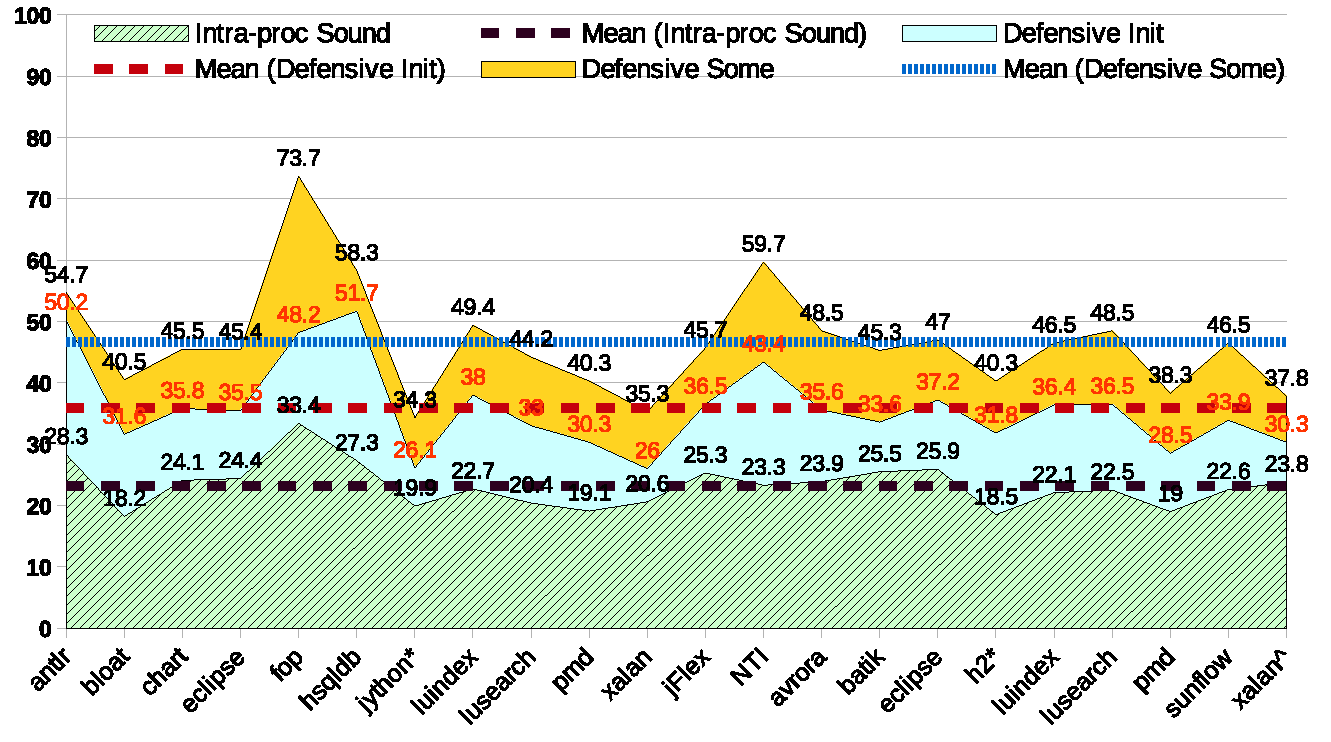
\includegraphics[width=\linewidth]{assets/defensive/vars.pdf}
\caption{Percentage of application variables (deemed reachable by baseline 2objH analysis) that have non-empty points-to sets for defensive analysis under some context and \ctxInit{} context (no assumptions). Intra-procedural sound points-to analysis (defensive minus the complex cases) shown as baseline. Arithmetic means are plotted as lines.}
\label{fig:sound:coverage}
\end{figure}

Thus, the defensive analysis achieves a large proportion of the benefits of an unsound analysis, while guaranteeing these results against uses of opaque code. We can answer \textbf{RQ1} affirmatively: defensive analysis covers a large part of realistic programs (over one-third unconditionally; close to one half under specific calling conditions), despite its conservative nature.


\paragraphhead{Comparison with intra-procedural.}
We have earlier referred to the ``easy'', intra-procedural parts of the analysis reasoning: what a compiler or VM would likely do to perform sound local data-flow analysis. This is the subject of \textbf{RQ2}, also answered by Figure~\ref{fig:sound:coverage}. The figure includes results for an intra-procedural baseline analysis that captures the low-hanging fruit of sound reasoning: local variables that directly or transitively (via ``move'' instructions) get assigned an allocated object. That is, the ``Intra-proc Sound'' analysis is otherwise the same as the full ``defensive'' logic, with the exception of the new ``interesting'' cases (control-flow merging, heap manipulation, and inter-procedural propagation). 

The result answers \textbf{RQ2} affirmatively: defensive analysis has significantly higher coverage than the baseline intra-procedural analysis. (And the difference only grows when considering an actual client, in later experiments.) Although the benefit is not broken down further in the figure, the handling of method calls alone (i.e., rules \infer{Call}, \infer{Args} and \infer{Ret}) is responsible for the lion's share of the difference between the full defensive analysis and the intra-procedural sound analysis.


%%% SPACE
%% Two data points in the experiment require further explanation. The
%% hsqldb benchmark is analyzed only partially by the underlying 2objH
%% analysis with the given reflection settings. Less than 10\% of the
%% statically available application code is deemed reachable.
%% % by 2objH, and is consequently also analyzed by 5def. 
%% The comparison of 2objH and 5def in this subset is still
%% meaningful, but may not be representative of the full complexity.
%% % of the hsqldb code. 
%% Also, for jython, 5def seems to cover 34.5\% of the application
%% variables produced by 2objH. However, this number is likely biased
%% (lowered) by the \emph{imprecision} of the unsound analysis: jython is
%% analyzed with a context-insensitive analysis, resulting in many
%% variables with spurious points-to sets.
%% % (See also later metrics on precision for jython.)
%% %
%% %If we allowed the 2objH
%% %analysis to complete (beyond a 3hr timeout) the real coverage of 5def
%% %would likely be higher for this benchmark. 

\paragraphhead{Running time.} 
Figure~\ref{fig:sound:time} shows the running times of the analysis, plotted next to that of 2objH, for reference. Although the two analyses are dissimilar, 2objH is qualitatively the closest one can get to defensive analysis with the current state of the art: it is an analysis with high precision, run with best-effort soundness support. Therefore, 2objH can serve as a realistic point of reference. As can be seen, the running times of defensive analysis are realistically low, although its flow-sensitive and 5-call-site-sensitive nature suggests it would be a prohibitively heavy analysis. This answers \textbf{RQ3} and confirms the benefits of laziness: a defensive analysis that only populates points-to sets once they are definitely bounded, achieves scalability for deep context.

\begin{figure}[tbh]
\centering
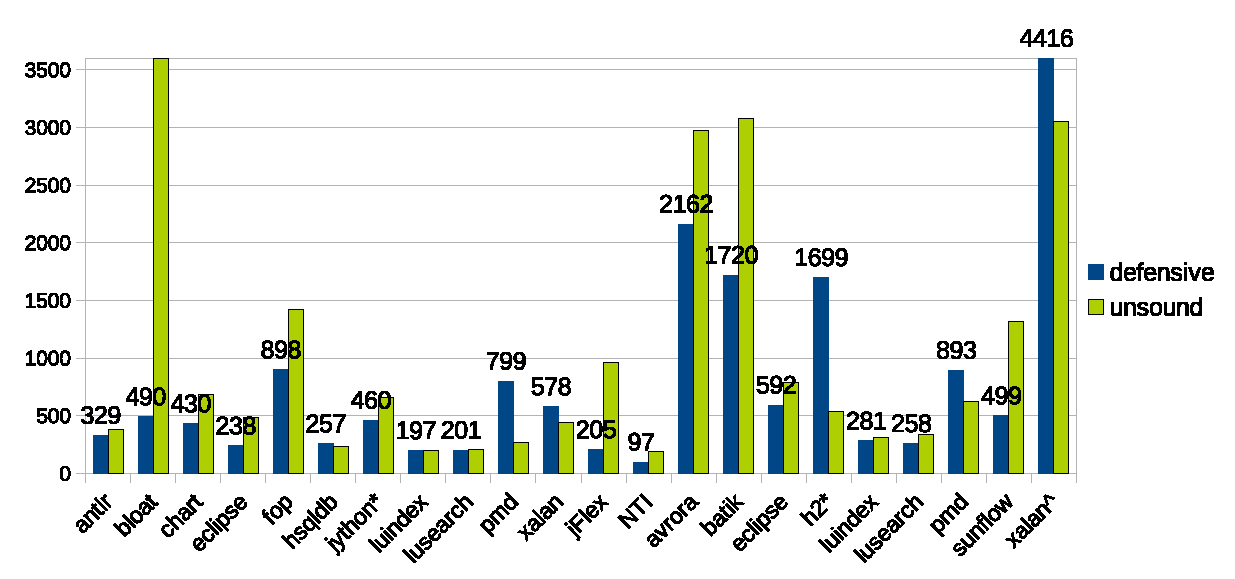
\includegraphics[width=\linewidth]{assets/defensive/time.pdf}
\caption{Running time (sec) of defensive analysis, with running time of 2objH (with unsound reflection handling) shown as a baseline. Labels are shown for defensive analysis only to avoid crowding the plot.}
\label{fig:sound:time}
\end{figure}


\paragraphhead{Client analysis: devirtualization.}
Our baseline analysis, 2objH, is highly precise and effective in challenges such as devirtualizing calls (resolving virtual calls to a single target method). On average, it can devirtualize \textbf{89.3\%} of the calls in the benchmarks studied (min: \bad{78.5\%}, max: \best{95.2\%}). However, these results are unsound and a compiler cannot act upon them. For optimization clients, such as devirtualization, soundness is essential. Using sound results, a JIT compiler can skip dynamic tests (of the inline caching optimization) for all calls that the analysis soundly covers.

Figure~\ref{fig:sound:devirt1} shows the virtual calls that defensive analysis devirtualizes, as a percentage of those devirtualized by the unsound analysis.

\begin{figure}[tbh]
\centering
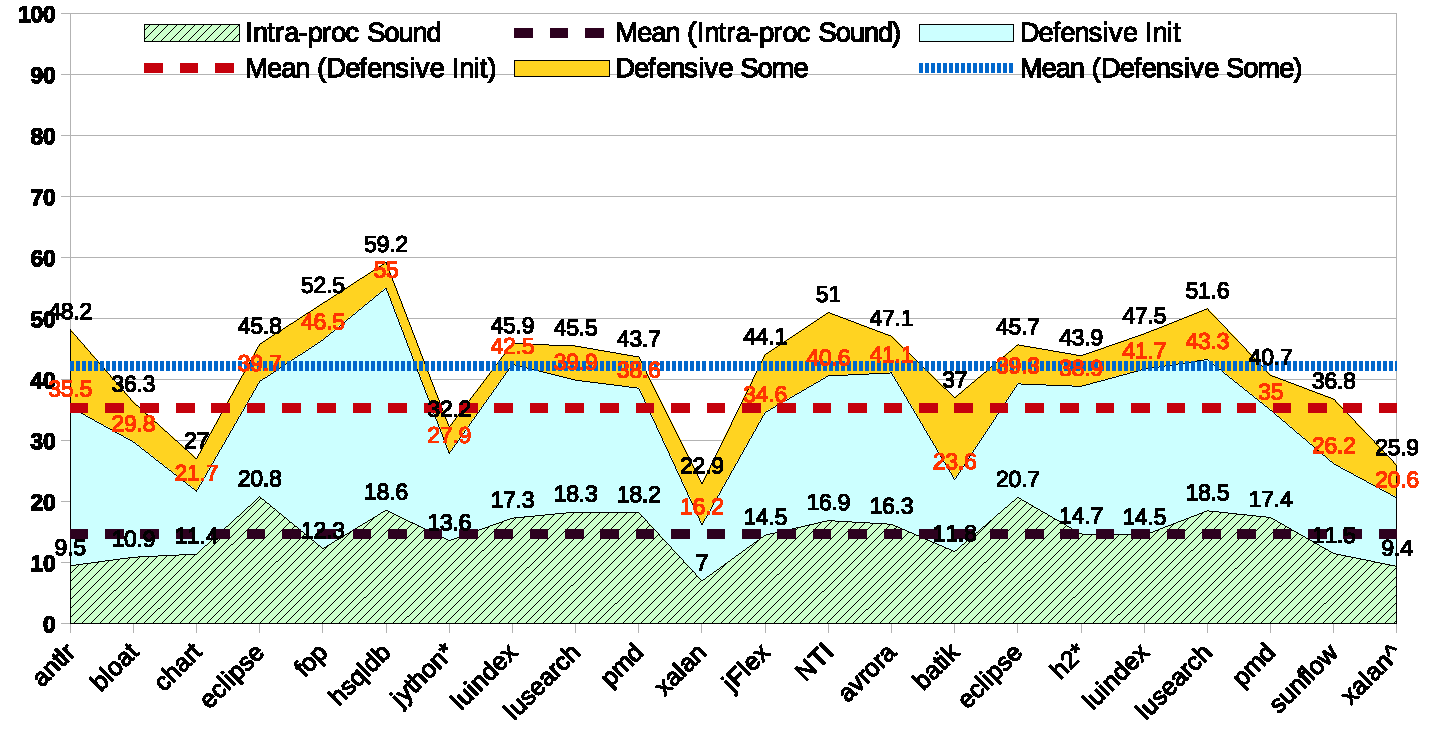
\includegraphics[width=\linewidth]{assets/defensive/devirt1.pdf}
\caption{Virtual call sites that are found to have receiver objects of a single type. These call sites can be soundly devirtualized. Numbers are shown as percentages of devirtualization achieved by unsound 2objH analysis.}
\label{fig:sound:devirt1}
\end{figure}

As can be seen, defensive analysis manages to recover a large part of the benefit of an unsound analysis (median \best{44.8\%} for optimization under a context guard, \textbf{38.7\%} for unconditional, \ctxInit{} context, optimization), performing much better than the baseline intra-procedural must-analysis (at 14.6\%). This answers \textbf{RQ4} affirmatively: the coverage of defensive analysis translates into real benefit for realistic clients.


\paragraphhead{Concurrency model.}
A compiler (JIT or AOT) author may (rightly) remark that the concurrency model of Section~\ref{sec:sound:assumptions} is not appropriate for automatic optimizations. The Java concurrency model permits a lot more relaxed behaviors, so the analysis is not sound for full Java as stated. However, the benefit of defensive analysis is that it starts from a sound basis and can add to it conservatively, only when it is certain that soundness cannot possibly be violated. Accordingly, we can remove the assumption that all shared data are accessed while holding mutexes, by applying the load/store rules only when objects trivially do not escape their allocating thread. We show the updated numbers for the devirtualization client (now fully sound for Java!) in Figure~\ref{fig:sound:devirt2}. The difference in impact is minimal: \best{43\%} of virtual call sites can be devirtualized conditionally, under some context, while \textbf{36\%} can be devirtualized unconditionally. This helps answer \textbf{RQ5}: defensive analysis can yield actionable results for a well-known optimization, under the Java memory model, for a large portion of realistic programs.

\begin{figure}[tbh]
\centering
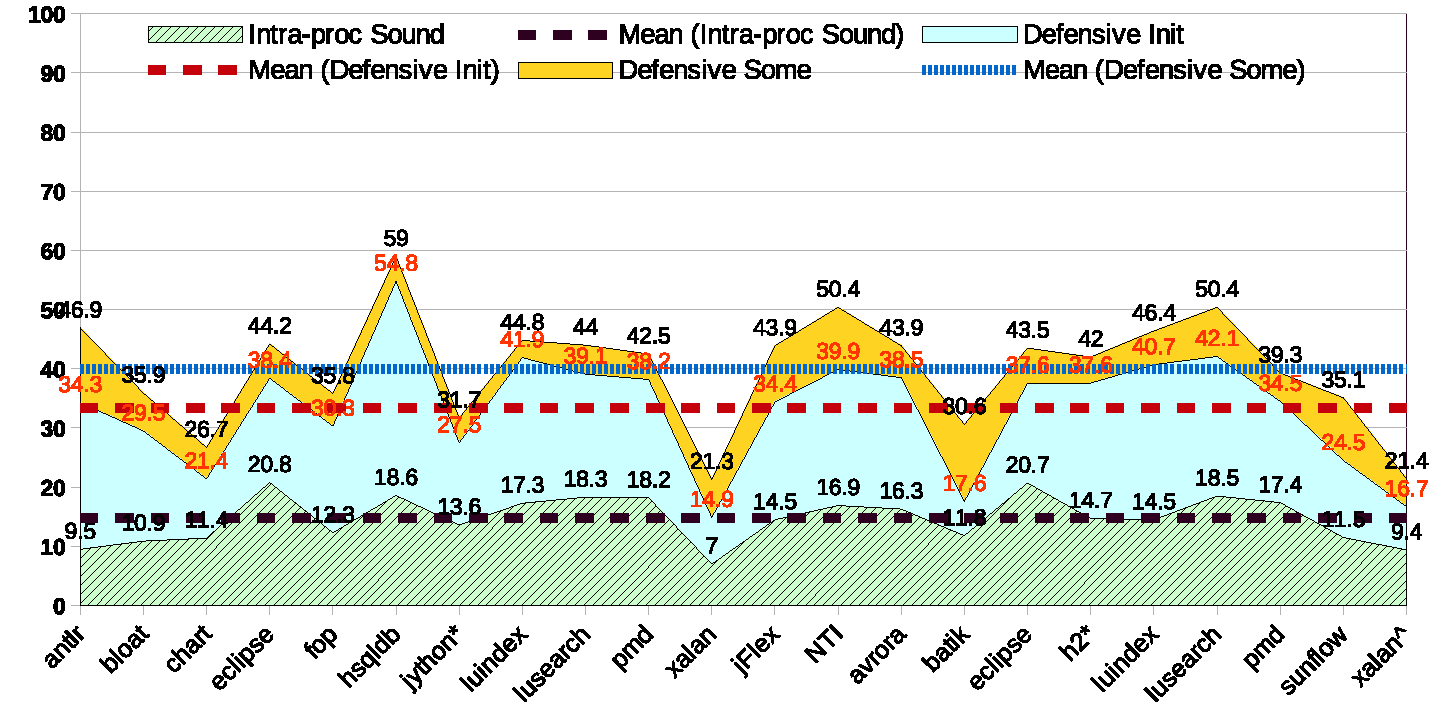
\includegraphics[width=\linewidth]{assets/defensive/devirt2.pdf}
\caption{Virtual call sites (percentage of 2objH) that are found to have receiver objects of a single type. Updates Figure~\ref{fig:sound:devirt1}, this time with soundness under a relaxed memory model.}
\label{fig:sound:devirt2}
\end{figure}


\paragraphhead{Points-to set sizes.}
Finally, it is interesting to quantify the precision of the defensive analysis, for the points-to sets it covers. This precision is expected to be high, since defensive analysis is flow- and context-sensitive, but exact figures help put it in perspective.

\begin{table*}[h!t]
\centering
\begin{tabular}{|c|l|cc!{\vrule width 2pt}cc|r|c|}
\cline{3-6}
\multicolumn{2}{c|}{} & defensive & 2objH & 2objH & defensive & \multicolumn{2}{c}{} \\
\cline{1-8}
\multirow{11}{0.4cm}{\rotatebox{90}{\mbox{DaCapo 2006-10-MR2}}}
& antlr     & 1.01  & 1.10  & 3.04  & 1.05  & avrora & \multirow{9}{0.4cm}{\rotatebox{90}{\mbox{DaCapo 9.12-Bach}}} \\
& bloat     & 1.02  & 2.12 	& 1.05  & 1.04  & batik & \\
& chart     & 1.09  & 1.09 	& 1.53  & 1.07  & eclipse & \\
& eclipse   & 1.06  & 1.31 	& 2.07  & 1.04  & h2* & \\
& fop       & 1.00  & 1.03 	& 1.04  & 1.01  & luindex & \\
& hsqld     & 1.01  & 1.04  & 1.08  & 1.03  & lusearch & \\
& jython*   & 1.01  & 6.05 	& 1.04  & 1.01  & pmd & \\
& luindex   & 1.02  & 1.02  & 1.08  & 1.05  & sunflow & \\
& lusearch  & 1.04  & 1.06 	& 1.19  & 1.04  & xalan\^ & \\
\cmidrule[2pt]{5-8}
& pmd       & 1.01  & 1.05 	& 1.02  & 1.01  & jFlex & \\
& xalan     & 1.05  & 1.12 	& 1.03  & 1.03  & NTI & \\
\cmidrule[2pt]{1-8}
\multicolumn{4}{|r|}{\textbf{``defensive'' mean}} & \multicolumn{4}{c|}{\best{1.03}} \\
\multicolumn{4}{|r|}{\textbf{``2objH'' mean}} & \multicolumn{4}{c|}{1.51} \\
\cline{1-8}
\end{tabular}
\caption[]{Average number of abstract objects pointed-by per variable, for variables for which both analyses compute results.}
\label{tab:sound:precision}
\end{table*}

Table~\ref{tab:sound:precision} shows average points-to set sizes for the defensive analysis vs. the 2objH analysis. The sets (excluding null values) are computed over variables covered by both analyses, for non-empty defensive analysis sets and under context \ctxInit{} of the defensive analysis, i.e., unconditionally. (The numbers are for the simplistic concurrency model, but remain unchanged to two significant digits for the relaxed concurrency model.)

As can be seen, the defensive analysis is highly precise when it produces non-empty points-to sets, typically yielding points-to set sizes very close to 1. 2objH is also a very precise analysis (for variables with bounded points-to sets), so it remains competitive, yet clearly less precise. Notably, points-to set sizes close to 1 are the Holy Grail of points-to analysis: such precision is actionable for nearly all conceivable clients of a points-to analysis.


\section{Summary}

Static analysis has long suffered from unsoundness for perfectly realistic language features, such as reflection, native code, or dynamic loading. We presented a new analysis architecture that achieves soundness by being \emph{defensive}. Despite its conservative nature, the analysis manages to yield useful results for a large subset of the code in realistic Java programs, while being efficient and scalable. Additionally, the analysis is modular, as it can be applied to any subset of a program and will yield sound results.

We expect this approach to open significant avenues for further work. The analysis architecture can serve as the basis of other sound analysis designs. The defensive analysis itself can be combined with several other analyses (may-escape, must-alias) that have so far been hindered by the lack of a sound substrate.